\documentclass[11pt, a4paper]{report}
\usepackage{graphicx}
\usepackage{float}
\usepackage{amsmath}
\usepackage{siunitx}
\usepackage{caption}
\usepackage{subcaption}
\usepackage[swedish]{babel}
\usepackage[utf8]{inputenc}
\usepackage{url}
\usepackage{graphicx}
\usepackage{pdfpages}
\usepackage[nottoc,numbib]{tocbibind}
\usepackage[utf8]{inputenc}
\usepackage[top=2.5cm, bottom=2.5cm, left=3cm, right=3cm]{geometry}
\usepackage[parfill]{parskip}

\usepackage{titlesec}

\titleformat{\chapter}[hang]   
{\normalfont\huge\bfseries}{\thechapter}{15pt}{\Huge}   
\titlespacing*{\chapter}{0pt}{0pt}{20pt}

\title{
\includegraphics{mah_logo.eps} \\[2 cm] Ingenjörsprojekt VT 2017 - Positioneringssystem}

\author{Gustaf Bohlin, Anton Hellbe, Mikael Nilsson, Arvid Sigvardsson}
\date{2017-05-29}

\begin{document}
\begin{titlepage}
\maketitle

\vfill
\begin{flushleft}
{\bf \underline{Email:}} \\
{\bf Anton} antonhellbe@gmail.com \\
{\bf Gustaf} gustaf.t.bohlin@gmail.com \\
{\bf Arvid} arvid.sigvardsson@gmail.com\\
{\bf Mikael} hellomicke89@gmail.com \\




\end{flushleft}
\centering  
\thispagestyle{empty}
\clearpage
\end{titlepage}

\chapter{Sammanfattning} 
Vi kommer här att göra en översiktlig beskrivning av arbetet
\begin{itemize}
\item Varför vi gör det, vad är målet med projektet?
\item har vi blivit begränsade på något sätt?
\item Hur blev resultatet? Motsvarar det förväntningar och krav?

\end{itemize} 
\newpage
\setcounter{page}{0}
\tableofcontents
\thispagestyle{empty}
\clearpage



\chapter{Inledning}
Här kommer vi att börja med att berätta  vad projektet går ut på samt att beskriva vad vår grupp har haft för uppgift under projektet.

Vi kommer göra en sammanställning av de vanligaste teknologierna som finns för inomhuspositionering idag. Vi kommer också att lista de idéer som vi själva brainstormat fram.
 


Förklara vad projektet kommer att handla om, varför projektet görs, vad målet med projektet är samt hypotes.

\chapter{Teori}

\section{Förstudie}

För att lösa problemet med robotens position inomhus har vi titta på lite olika lösningar för så kallade inomhus positionerings system. Inomhus positioneringssystem (IPS) används för att bestämma positionen på objekt eller personer inomhus. Exempel på  tekniker som används för detta är Radiovågor(UWB), Ljud(ultraljud), WiFi/Bluetooth signalstyrkor och s.k Dead reckoning (Dödräkning med hjälp av Gyroskop / Accelerometer)


UWB(Ultra WideBand Technology): \\
Ultra wideband är en teknik för WPAN. Detta är en väldigt förekommande teknik för inomhus positioneringssystem på grund av att postionen blir väldigt exakt jämfört med många andra tekniker. UWB använder sig av radiovågor som rör sig i ljusets hastighet vilket betyder att man behöver väldigt exakta tidpunkter för att bestämma var objektet / personen befinner sig. För att bestämma positionen används TDoA (Time Difference of Arrival) algoritmer för att ta reda på tiden det tog för signalen att komma fram. Tiden används sedan vid triangulering för att få fram positionen.

När det kommer till sändare och mottagare kan man låta sändarna ta emot signalen som har studsat på objektet. Detta innebär att inga komponenter krävs på roboten men för att få ''rätt'' signal på mottagarsidan behöver man kolla på fasen för att kunna utesluta fading.

Ultraljud: \\
Ultraljud är ljudvågor som är över $20\textrm{kHz}$, dvs ljud som människan ej kan höra. Fördelen med Ultraljud är att ljud rör sig i $340\textrm{m/s}$ jämfört med ljusets hastighet $3 \cdot 10^{8}\textrm{m/s}$. För att ta fram avståndet till en fyr använder man formeln
\begin{equation}
s = v \cdot \Delta t
\end{equation}
Med en mindre $v$ kan sträckan beräknas noggrannare. Positionen på objektet/personen kan sedan räknas ut med hjälp av triangulering.

Dead Reckoning:\\
Dead reckoning eller död räkning på svenska går ut på att med hjälp av en accelerometer och ett gyroskop så kan man bestämma positionen. Detta görs genom att känna till start positionen och sedan med hjälp av datan från gyroskopet (orientationen) och accelerometern (accelerationen) så kan man beräkna hur objektet / personen har rört sig genom integration och  på så sätt dess position. Det är en elegant lösning från den synvinkeln att det inte kräver några utomstående komponenter men problemet är att om det uppstår fel i mätdatan så kommer felet kvarstå. Detta betyder att man regelbundet skulle behöva kalibrera om för att undvika för mycket kvarstående fel.

WiFi / Bluetooth signalstyrkor: \\

Genom att placera ut noder t ex 3 eller 4 så kan man mäta upp RSSI (Recieved Signal Strength Indication) detta gäller både WiFi och Bluetooth och med hjälp av den uppmätta signalstyrkan till de olika noderna sedan bestämma positionen. Problemet med detta är att noggranheten är väldigt dålig, ofta handlar det om flera meter vilket är oacceptabelt om roboten skall kunna navigera fram till objekt.

\begin{center}
     \begin{tabular}{l | c | c}
  		Teknik & Fördelar & Nackdelar \\ \hline
        Ultrawideband & Bra noggrannhet & Dyr\\
         & Arduino bibliotek \\ \hline
        Ultraljud & Bra noggrannhet & Inget bibliotek\\
        & Billigt & Möjligtvis problem med resonans\\
        & Låga krav på hårdvaran \\ \hline
        Dead Reckoning & Enkelt & Dålig noggrannhet \\
        & Billig & Integrerande fel \\ \hline
        Bluetooth / WiFi & Enkelt & Dålig noggrannhet \\
        & Använt på tidigare laborationer
  \end{tabular}
  \end{center}


Vad har vi fått reda på för information när vi har undersökt problemet, vilka olika lösningar som har disskuterats. 

\chapter{Metod och utförande}

För att bestämma vilken teknologi som kommer att användas till inomhus positionering systemet måste problemet formuleras och krav måste anges. Problemet som skall lösas definieras enligt följande: \\

''Vi vill hitta positionen på ett objekt i ett rum. Positionen skall faställas i ett 2D plan. Eftersom en robot skall kunna hitta till olika objekt  i ett rum behöver den känna till sin position vid given tidpunkt. Objekten kommer att vara mindre hushållsobjekt.'' \\

När problemet är givet kan behov för lösningen definieras. De behov som systemet skall ha är följande:

\begin{itemize}
	\item Positionen skall kunna fastställas i realtid.
	\item Noggrannhet skall vara tillräcklig för att armen skall kunna nå objektet.
	\item Systemet skall kunna användas i en offentlig miljö.
	\item Systemet skall fungera i en begränsad plan yta.
	\item Systemet skall fungera oberoende av ljusförhållanden.
	\item Systemet skall ha ett rimligt pris.
	\item Systemet skall kunna kommunicera med roboten.
	\item Systemet för ej vara skadligt.
	\item Systemet får ej vara opålitligt.
\end{itemize}

Härnäst skapas en tabell där behoven uttrycks i egenskaper med mätbara enheter.

\begin{center}
     \begin{tabular}{l | c}
  		Positionen skall fastställas med ett intervall & Hz \\ \hline
        Hög noggrannhet & cm\\ \hline
        Ofarlig & subjektiv\\ \hline
        Möjlig att integrera & subjektiv\\ \hline
        Områden anges med riktlinjer av något slag & subjektiv \\ \hline
        Systemet fungerar i varierande ljusförhållanden & lm \\ \hline
        Inom skolans budget & kr \\ \hline
        Systemet har ett överföringsprotokoll till roboten & subjektiv
  \end{tabular}
\end{center}
\cleardoublepage
För att säkerställa att alla behoven har uppfyllts av egenskaperna skapas en behov-egenskap matris.

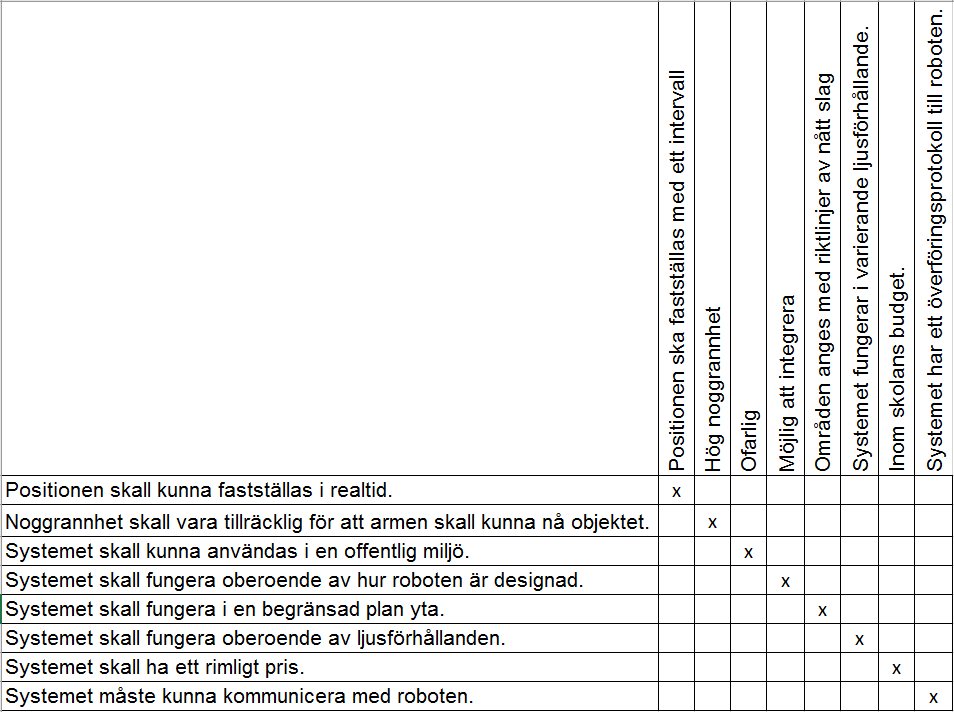
\includegraphics[scale=0.5]{behov-egenskap-matris.PNG}\\
fig \ref{fig:behov-egenskap} \textit{Behov-egenskap matris} %varför är det 9.1???

Som man ser i matrisen uppfylls alla behoven av egenskaperna och därmed är det känt vad en lösning kommer att behöva.

%Systembegrepp bild??


Här kommer vi att beskriva hur vi har gått tillväga för att nå ett resultat. Hur har vi kommit fram till vilken teknologi vi kommer att använda?

Hur har vi gått till väga för att konstruera valt positioneringssystem?
Vilka resurser har vi använt oss av?

\section{Syfte och mål för vår tekniska lösning}
Syftet med den tekniska lösningen är att roboten skall veta var den befinner sig.

Målet med den tekniska lösningen är positionen inte skiljer sig från robotens faktiska position.

\section{Systemkrav}
För att utveckla en produkt, i vårt fall ett positioneringssystem, krävs det att innan man börjar sätter upp ett antal krav som man vill att produkten ska uppfylla. Uppgiftsbeskrivningen listar ett fåtal krav och vi har genom diskussion kommit fram till följande kravspecifikation:
\begin{itemize}
\item Positionen skall kunna fastställas i realtid.
\item Noggrannhet skall vara tillräcklig för att armen skall kunna nå objektet.
\item Systemet skall kunna användas i en offentlig miljö.
\item Systemet skall fungera oberoende av hur roboten är designad.
\item Systemet skall fungera i en begränsad plan yta.
\item Systemet skall fungera oberoende av ljusförhållanden.
\item Systemet skall ha ett rimligt pris.
\item Systemet skall kunna kommunicera med roboten.

\end{itemize}
 Dessa kan sedan översättas till en lista som är är mer lämpad att arbeta utefter:
 \begin{center}
     \begin{tabular}{ c | c}
     	Mätbar Egenskap & Enheter  \\ \hline
  		Positionen ska fastställas med ett visst intervall & Hz  \\ \\
        Hög noggrannhet & cm\\ \\ 
        Ofarlig & subj. \\ \\
        Möjlig att integrera & subj.\\ \\
        Områden följer förutbestämda riktlinjer & subj\\ \\
        Systemet ska fungera i varierade ljusförhållanden & lm\\ \\
        Kostnaden ska täckas av skolans budget & kr  \\ \\
        Systemet har ett överföringsprotokoll till roboten & subj.\\ 

  \end{tabular}
  \end{center}

Vi kan nu sätta ihop dessa i en s.k. behov-egenskapsmatris som kan ses i bilaga \ref{fig:behov-egenskap}
\section{Problembeskrivning}
Vi vill hitta positionen på ett objekt i ett rum. Positionen skall fastställas i ett 2D plan. Eftersom en robot ska kunna hitta till olika objekt i ett rum behöver denna känna till sin position vid given tidpunkt. Objekten kommer att vara mindre hushållsobjekt.

Vi har i teoriavsnittet tagit upp hur liknande, fast etablerade system, fungerar. Det som skiljer de systemen från vårt är att vårt system har väldigt specifikt användningsområde. Vårt system ska t.ex. inte användas i totalt mörker. Ytan är inte heller dynamisk ytan noga uträknad för att kalibrera systemet. Det är alltså inte troligt att vårt system, utan större vidareutvecklingar, hade fungerat i t.ex. ett varuhus. Vi har även endast en användare vilket förenklar positioneringen något.

Vi har identifierat systemets in- och utgångar och visualiserar det i figur \ref{fig:system-omgivning}
\begin{figure}[H]
	\begin{center}
		\includegraphics [width=12cm,angle=0]{system-omgivning.png}
		\caption{Illutration av systemets in- och utgångar samt dess omgivning}
		\label{fig:system-omgivning}
	\end{center}
\end{figure}

Omgivningen påverkar systemet om det är objekt i vägen då alla ingångar förutom acceleration, rotation påverkas av detta. Systemet påverkas även av störande signaler i omgivningen. Systemets påverkan på omgivningen är i många fall att den skickar ut signaler som stör andra signaler




\chapter{Resultat}
Vi kommer att klargöra vilka teknologi/er vi har valt för vår lösning och varför som resultat av vår konceptstudie.

Beskrivning av hur, vårt nu fungerande positioneringssystem, fungerar. 

\chapter{Diskussion}
\begin{itemize}
\item Vad gick bra, vad gick som vi hade tänkt oss?
\item Hur fungerar vårt system jämfört med andra som finns och varför?
\item Hade det gått att använda vårt system i större skala?
\end{itemize} 




\chapter{Slutsats}
Vi gör här en kort summering av arbetet.
Samt:
Vilka slutsatser kan vi dra från resultatet och projektet i stort?
Vad har vi lärt oss?






\newpage
\begin{thebibliography}{99}

\bibitem{Tom} Tom

\end{thebibliography}

\chapter{Bilagor}
Vi kommer här att lägga bilder och ekvationer samt eventuella länkar som hindrar läsbarheten och bara tar plats i texten.

\begin{figure}[H]
	\begin{center}
		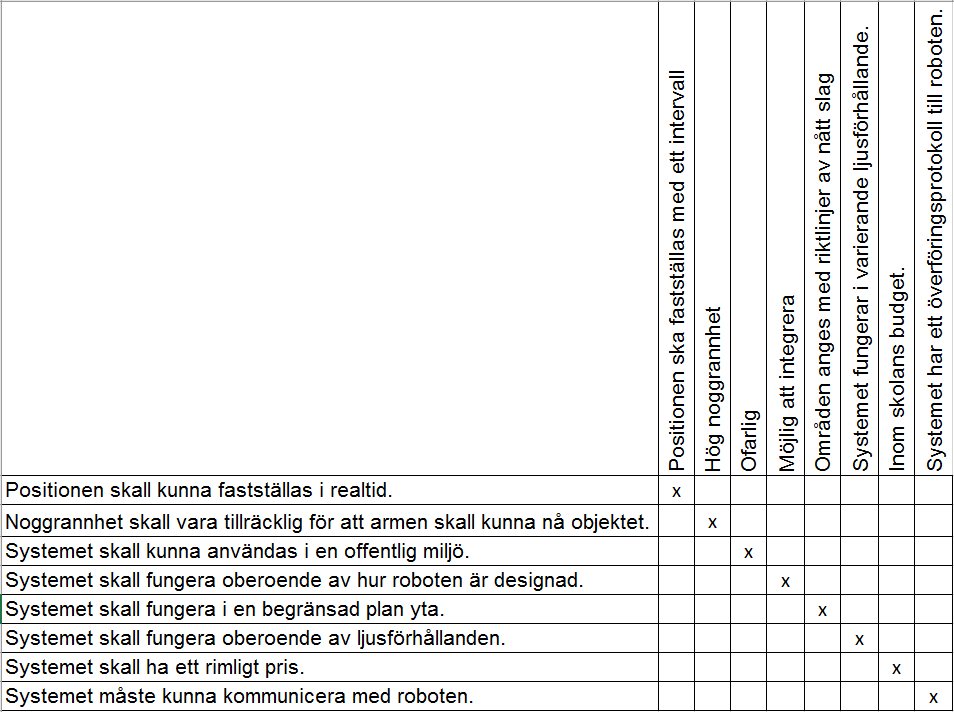
\includegraphics [width=12cm,angle=0]{behov-egenskap-matris.png}
		\caption{Behov-egenskapsmatris}
		\label{fig:behov-egenskap}
	\end{center}
\end{figure}
\end{document}

